\documentclass{article}
\usepackage{graphicx} % Required for inserting images
\usepackage{tikz}
\usetikzlibrary{graphs} % LaTeX and plain TeX
\usepackage{algorithm}
\usepackage{algpseudocode}

\title{Übung 1 für Mathe IT-1}
\author{Jean-Pierre Kasperschinski, Max Derno, Boban Petrov}
\date{20.10.2024}

\begin{document}
\maketitle

\section*{1. Aufgabe}

    \subsection*{a)}
    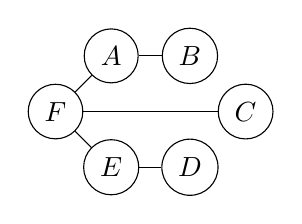
\begin{tikzpicture}[main/.style = {draw, circle}]
    \node[main] (1) {$A$};
    \node[main] (2) [right of=1] {$B$};
    \node[main] (3) [below right of=2] {$C$};
    \node[main] (4) [below left of=3] {$D$};
    \node[main] (5) [left of=4] {$E$};
    \node[main] (6) [above left of=5] {$F$};

    \draw (1) -- (2);
    \draw (1) -- (6);
    \draw (3) -- (6);
    \draw (5) -- (6);
    \draw (4) -- (5);
    \end{tikzpicture} \newline
    Das billigste Netz sieht aus wie in dieser Grafik und kommt dabei auf Kosten von 126 Geldeinheiten, um dieses zu erstellen habe ich mir aus der Tabelle in der Zeile mir die niedrigste Zahl gesucht und dann die ensprechende Spalte kontrolliert ob es keinen niedriegeren Betrag gibt

    \subsection*{b)}
    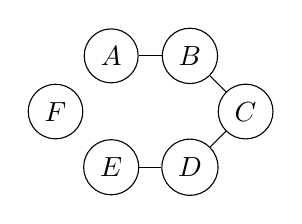
\begin{tikzpicture}[main/.style = {draw, circle}]
    \node[main] (1) {$A$};
    \node[main] (2) [right of=1] {$B$};
    \node[main] (3) [below right of=2] {$C$};
    \node[main] (4) [below left of=3] {$D$};
    \node[main] (5) [left of=4] {$E$};
    \node[main] (6) [above left of=5] {$F$};

    \draw (1) -- (2);
    \draw (2) -- (3);
    \draw (3) -- (4);
    \draw (4) -- (5);
    \end{tikzpicture} \newline
    Meiner Meinung war dies keine Gute entscheidung, da es nun 127 Geldeinheiten sind (also teurer) und eine Stadt weniger an das Netz angeschlossen wurde
\newpage
\section*{2. Aufgabe}

    \begin{algorithm}
    \caption{istTeilbar}\label{alg:cap}
    \begin{algorithmic}
    \Require $x,y$
    \Ensure $Boolean$
        \While{$x \geq y$}
            \State $x = x - y$
        \If{$x = 0$} {
        true} \Else{
        false
        }
    \end{algorithmic}
    \end{algorithm}\newline
    Es werden ein x und y Wert eingegeben und man erhält als Ergebnis ein Boolean, je nachdem ob es Teilbar ist oder nicht (true = Teilbar, false = nicht Teilbar)
    

\section*{3. Aufgabe}

    

    \subsection*{a)} 
    $\frac{n+1}{2n} + \frac{3n+1}{5n} + \frac{4n+3}{10n} = \frac{15n+10}{10n} = \frac{3n+10}{2n}$
    \subsection*{b)}
    $\frac{n}{2^n} - \frac{n+1}{2^n+1} - \frac{n+2}{2^n+2} = \frac{1}{2^n} * (n - \frac{n+1}{2} - \frac{n+2}{4}) = \frac{n-4}{4*2^n}$
    \subsection*{c)}
    $\frac{(n+1)-(1-n)}{n*(n+1)} = \frac{2n}{n*(n+1)} = \frac{2}{n+1}$
    \subsection*{d)}
    $\sqrt{\sqrt[3]{\sqrt[4]{16n}*32}+4} = \sqrt{\sqrt[3]{\sqrt[4]{n}*64}+4} = \sqrt{\sqrt[12]{n}*4+4}$
    \newline
    $ = 2 * \sqrt{\sqrt[12]{n}+4} = 2 * \sqrt[24]{n}+2$
    \subsection*{e)}
    $(n+1)^k * (\frac{1}{n-1})^l * (\frac{n-1}{n+1})^k * \sqrt[k]{(n-1)^l} =$ \newline
    $(n-1)^k * (n-1)^{-l} * (n-1)^{\frac{l}{k}} =$ \newline
    $(n-1)^{\frac{l}{k} + k - l}$ \newpage
    \subsection*{f)}
    $(\log_{n}(k+1)) * (\log{42}(\sqrt[\log_{42}(k+1)]{n}))$ \newline
    $(\log_{n}(k+1)) * (\log{42}(n^{\frac{1}{\log_{42}(k+1)}})$ \newline
    $(\log_{n}(k+1)) * (\log{42}(n) * \frac{1}{\log_{42}(k+1)}$ \newline
    $\frac{\log_{42}(k+1)}{\log_{42}(n)} * \frac{\log_{42}(n)}{\log_{42}(k+1)} = 1$

\section*{4. Aufgabe}

    \subsection*{a)}
    $11n +16k = 6m + 7n$ \newline
    $n= \frac{3}{2}m - 4k$
    \subsection*{b)}
    $3n + k = 7m(n-1)$ \newline
    $n = \frac{-7m-k}{3-m}$
\end{document}

